% !TeX root = project-report-B-cn.tex
% !TeX program = lualatex
% Build: latexmk -lualatex -interaction=nonstopmode -halt-on-error -outdir=.build/project-report-B-cn project-report-B-cn.tex
\documentclass[11pt,a4paper,fontset=fandol,scheme=plain]{ctexart}
\usepackage[margin=21mm,headheight=14pt]{geometry}
\usepackage{lmodern,amsmath,amssymb,graphicx,booktabs,array,tabularx}
\usepackage{xcolor,enumitem,fancyhdr,caption,xurl,placeins,float,needspace}
\usepackage[colorlinks=true,linkcolor=teal,citecolor=teal,urlcolor=teal]{hyperref}
\definecolor{reportblue}{HTML}{18536B}
\hypersetup{pdftitle={四轻子神经网络研究进展：筛选效果、输入组比较与统计可靠性},pdfauthor={HiggsML 项目}}
\pagestyle{fancy}
\fancyhf{}
\fancyhead[L]{\small\textcolor{reportblue}{HiggsML | 项目报告}}
\fancyhead[R]{\small 2026 年 11 月 1 日}
\fancyfoot[C]{\thepage}
\setlength{\parindent}{0pt}
\setlength{\parskip}{6pt}
\setlength{\emergencystretch}{2em}
\setlist[itemize]{leftmargin=1.4em,itemsep=3pt,topsep=4pt}
\captionsetup{font=small,labelfont=bf,justification=raggedright,singlelinecheck=false}
\captionsetup[table]{name=表}
\captionsetup[figure]{name=图}
\newcolumntype{Y}{>{\raggedright\arraybackslash}X}
\ctexset{
  section={format=\Large\bfseries\color{reportblue},beforeskip=16pt,afterskip=8pt},
  subsection={format=\large\bfseries\color{reportblue},beforeskip=12pt,afterskip=5pt}}
\setcounter{tocdepth}{1}
\renewcommand{\contentsname}{阅读目录}
\raggedbottom
\setlength{\textfloatsep}{12pt}
\setlength{\intextsep}{12pt}
\newcommand{\gev}{\,\mathrm{GeV}}

\begin{document}
{\LARGE\bfseries\color{reportblue} 四轻子神经网络研究进展：筛选效果、输入组比较与统计可靠性\par}
\vspace{6pt}
项目报告 · 问题驱动版 · 2026 年 11 月 1 日

\section{研究问题与主要发现概览}

本报告按三个问题组织已有研究：网络选择了哪些事件，删去输入组后标称区间怎样变化，以及这些差异有多稳健。
每个问题先给出理解结果所需的方法，再展示证据，最后说明结论能够支持到什么程度。

\begin{center}
\small
\begin{tabularx}{\linewidth}{@{}p{.23\linewidth}Y@{}}
\toprule
问题 & 当前发现与边界 \\
\midrule
网络筛选效果 & 两个示例网络保留大部分信号、压低约一半背景；背景谱形也变化，不能只看总保留率。 \\
输入组作用 & 删去 C 的标称区间在三个种子中均变宽；其余删组差值随种子改变符号。 \\
差异的稳健性 & 固定网络下的重抽样支持 C 的变宽方向；model-self 检验存在欠覆盖，尚无独立校准。 \\
\bottomrule
\end{tabularx}
\end{center}
全部结论限于探索性、非独立的教育用途 MC 研究，不构成 ATLAS/CMS 官方结果、希格斯发现或物理测量。

\section{共同背景与研究比较基础}

\subsection{样本与共同选择}
分析使用 ATLAS 2020 教育用途 13 TeV 集合的两份 MC 样本\cite{OpenData}，产额对应
$10\,\mathrm{fb}^{-1}$。信号 DSID 345060（\texttt{ggH125\_ZZ4lep}）表示胶子融合产生
质量设为 $125\gev$ 的希格斯，再经 $H\to ZZ^*\to4\ell$ 衰变。背景 DSID 363490
（\texttt{llll}）为四轻子样本；具体初态及 $Z/\gamma^*$ 贡献尚缺 DSID 生产说明，不能将其写成纯夸克初态 $ZZ$。
本项目另选 $2e2\mu$ 末态，这不是对生成样本末态范围的声明。
所有比较使用同一共同选择：先检查事件触发和轻子品质，再要求恰好四个合格轻子，
构造同味异号轻子对，施加动量、接受度与轻子对质量条件，最后限制为
$2e2\mu$ 末态及 $105\leq m_{4\ell}<140$ GeV。
电子对和缪子对组成两个候选；质量更接近 $91.1876$ GeV 的一对称为 $Z_1$，另一对为 $Z_2$。
这里的重建是对公开轻子四动量作组合，不是重新模拟探测器。
完整条件、执行顺序和文献对应见附录~\ref{app:cuts}，四动量与角度定义见附录~\ref{app:fields}。

“网络筛选前”已经通过这些共同条件；“网络筛选后”仅额外要求通过固定网络的高分阈值。
因此，两者是同一评估总体与其中的子集，不是独立产生的两批事件。

\subsection{输入组、样本分工与冻结规则}

输入由轻子四动量构造，分为四组：A 为单轻子运动学（8 维），B 为轻子对质量与角分离（4 维），
C 为四轻子系统及两个轻子对的整体运动学（2 维），D 为五个角度（5 维）。
ABCD 使用全部 19 维；BCD 去掉 A，使用 11 维。完整研究还训练 ACD、ABD、ABC，分别为 15、17、14 维。
每一种表示均单独训练，而不是在同一个已训练网络中把某组输入置零。

所有分类器均不显式输入 $m_{4\ell}$，但各输入共享底层轻子信息、彼此相关，仍可能携带质量信息。
因此，后文需要直接检查筛选后的质量谱，不能仅凭“未输入质量”断言选择与质量无关。

共同选择后的事件按物理事件组，以 60\%、20\%、20\% 的概率分别分配到训练、验证和最终评估子集。
同组事件始终在同一子集，所有输入方案和种子共用这一分配。比例是分配概率，实际计数不必恰好等于该比例。

\begin{center}
\small
\begin{tabularx}{\linewidth}{@{}p{.14\linewidth}p{.18\linewidth}Y@{}}
\toprule
子集 & 分配概率 & 在本研究中负责什么 \\
\midrule
训练 & 60\% & 拟合输入标准化参数与网络参数。 \\
验证 & 20\% & 用 AUC 选择检查点，再用背景分数确定阈值。 \\
最终评估 & 20\% & 在模型与阈值冻结后，计算产额、质量谱及区间结果。 \\
\bottomrule
\end{tabularx}
\end{center}
评估结果不回流到模型选择或阈值调节。此处的流程分工不等于源样本独立：研究重新使用了此前已使用过的 MC 事件。

\Needspace{13\baselineskip}
\subsection{三个不同层次的量：事件数、产额与区间宽度}

\label{sec:weights}
事件组数回答“有多少模拟样本”，带符号权重之和回答“给定亮度下预期有多少事件”。
两者不是同一个量：大量 MC 事件可以只对应少量预期产额。
令 $w_i^{\rm phys}$ 为样本归一化后的物理权重；最终评估只使用分配概率为 0.2 的子集，故其产额权重为
\[
 u_i=\frac{w_i^{\rm phys}}{0.2},\qquad
 Y_{\rm before}=\sum_{i\in E}u_i,\qquad
 Y_{\rm high}=\sum_{i\in E,\,s_i\geq t}u_i,\qquad
 R=\frac{Y_{\rm high}}{Y_{\rm before}}.
\]
这里 $E$ 表示某一过程的最终评估基线事件，$s_i$ 是网络分数，$t$ 是该模型的冻结阈值，$R$ 是产额保留率。
除以 0.2 用于估计同一 $10\,\mathrm{fb}^{-1}$ 下的产额；训练、验证和评估子集不能作为三份独立亮度相加。
负生成器贡献保留原符号。物理归一化公式与样本常数见附录~\ref{app:weights}。

第三个量是 $W_{68}=\mu_{\rm upper}-\mu_{\rm lower}$，表示标称 68\% 信号强度区间的宽度；
$\mu$ 缩放预期信号产额。它来自似然推断，既不是网络 AUC，也不是信号保留率。
因此，分类排序更好或某张谱图更突出，都不能直接证明区间更窄或覆盖率更可靠。

\FloatBarrier

\section{神经网络筛选效果与保留样本}

先固定一条由训练和验证决定的选择规则，再问它在最终评估样本上留下什么。
本章使用种子 42 的 ABCD、BCD 两个模型；完整输入组比较在下一章给出。

\subsection{先学习分数，再选择检查点}

训练的目标是给信号事件较高分数、给背景事件较低分数。信号标签设为 1，背景标签设为 0。
首先只在训练集计算每个输入的均值与标准差，再将同一标准化变换应用于验证和评估样本。
网络把每个事件的输入映射为 $0$--$1$ 分数 $s$；分数越高越倾向于信号，但它不是已校准的物理信号概率。

每轮训练用加权二元交叉熵衡量分数与标签的差异，再通过反向传播和 AdamW 更新参数。
用于优化的权重取物理权重的绝对值，并除以所属训练类别的平均绝对权重；这不强制两类的总权重相等。
训练权重服务于参数学习，最终产额则使用带符号物理权重，两者用途不同。

每轮训练后，在验证集上用绝对物理权重计算 AUC（ROC 曲线下面积），检查信号是否通常排在背景之前。
AUC 为 0.5 表示随机排序水平，1 表示完全区分。AUC 用于比较同一训练过程中的检查点，不负责设定高分阈值。

只有验证 AUC 比此前保存的最佳值提高超过 $10^{-4}$，才保存新检查点；
连续 20 轮没有这样的改进就提前停止，最多训练 200 轮。停止后恢复保存的最佳检查点，
因此“结束训练的轮次”与“最终使用的轮次”可以不同。
例如种子 42 的 ABCD 在第 87 轮停止、使用第 67 轮；BCD 在第 86 轮停止、使用第 66 轮。
网络结构与超参数见附录~\ref{app:network}。

\Needspace{13\baselineskip}
\subsection{确定阈值并冻结选择}

模型确定后，还需要一条规则把连续分数分为高分和低分。每个模型只使用\emph{验证集背景}确定自己的阈值，步骤为：
\begin{enumerate}[leftmargin=1.7em,itemsep=2pt,topsep=3pt]
\item 将验证背景按网络分数从小到大排序。
\item 累加每个事件的绝对物理权重，找到累计权重第一次达到总权重一半的位置。
\item 将该位置的实际分数记为阈值 $t$；不在相邻分数之间插值。
\end{enumerate}
因此，这是一条预先规定的加权中位数规则，不是扫描最终评估样本以寻找最佳筛选效果。
应用时，$s\geq t$ 的事件进入高分类别，$s<t$ 的事件进入低分类别；同分事件不拆开。

种子 42 的实际阈值为 ABCD 的 $0.746724$ 和 BCD 的 $0.860891$（此处舍入展示，评估使用原始精度）。
两个网络的分数刻度不同，不能仅凭阈值数值的大小判断哪个网络更好。

输入标准化参数、网络检查点和分数阈值全部冻结后，才将它们应用于最终评估样本。
每个基线事件先得到分数，再按阈值划入高分或低分类别；随后分别计数、求带符号权重和并绘制质量谱。
原始事件的质量值没有被网络改写，改变的是哪些事件进入展示的高分子集。

加权中位数规则不保证背景恰好保留 50\%。首先，离散权重和同分事件会使验证集高分绝对权重占比偏离一半；
其次，最终评估是另一个子集，且产额保留率使用\emph{带符号}权重。
附录~\ref{app:threshold} 给出一个明确标为教学示例的计算。

本文的高分谱用于解释筛选效果。后续区间推断仍使用高分和低分两个类别，
各类别均在整个 $[105,140)$ GeV 区间内积分；图中的七个质量箱仅用于展示，不是推断分箱。

\subsection{事件数与预期产额的变化}

固定模型、阈值与评估总体后，表~\ref{tab:groups} 比较基线与高分子集的物理事件组数。
\begin{table}[H]
\caption{最终评估样本中的物理事件组数。后两列为种子 42 的高分子集，并非新的独立样本。}
\label{tab:groups}
\centering
\small
\begin{tabular}{lrrr}
\toprule
过程 & 基线（网络筛选前） & ABCD 高分 & BCD 高分 \\
\midrule
信号 & 9,049 & 8,761 & 8,563 \\
背景 & 698 & 386 & 378 \\
\bottomrule
\end{tabular}
\end{table}
例如，8,761/9,049 是 ABCD 的信号事件组保留比例；96.80\% 是带符号产额保留率，两者不同。
\begin{table}[H]
\caption{$10\,\mathrm{fb}^{-1}$ 下的预期带符号产额及保留率。
误差为固定网络和阈值下按物理事件组计算的 MC 标准误差；保留率误差包括筛选前后共享事件的协方差。}
\label{tab:yields}
\centering
\small
\begin{tabular}{llrr}
\toprule
过程 & 选择 & 预期产额 & 保留率（\%） \\
\midrule
信号 & 筛选前 & $2.7710\pm0.0293$ & --- \\
 & ABCD 高分 & $2.6824\pm0.0288$ & $96.80\pm0.19$ \\
 & BCD 高分 & $2.6215\pm0.0285$ & $94.60\pm0.24$ \\
背景 & 筛选前 & $2.3553\pm0.1683$ & --- \\
 & ABCD 高分 & $1.2027\pm0.1202$ & $51.06\pm3.57$ \\
 & BCD 高分 & $1.1012\pm0.1156$ & $46.75\pm3.57$ \\
\bottomrule
\end{tabular}
\end{table}
ABCD 保留 96.80\% 的信号产额和 51.06\% 的背景产额，即约损失 3\% 的信号、去除 49\% 的背景；
BCD 分别保留 94.60\% 和 46.75\%，即约损失 5\% 的信号、去除 53\% 的背景。
保留率是同一过程筛选后与筛选前的带符号产额之比，不是平均网络分数。

BCD 在自身阈值下同时去除更多信号和背景。这不是等信号效率比较，不能据此判断网络优劣。

\FloatBarrier

\clearpage
\subsection{绝对质量谱与各质量区域的筛选效果}
图~\ref{fig:yields} 展示神经网络筛选前后的不变质量分布。左列为模拟希格斯信号，右列为背景。
每个面板在相同亮度和质量分箱边界下，比较基线与其高分子集。

\begin{figure}[H]
\centering
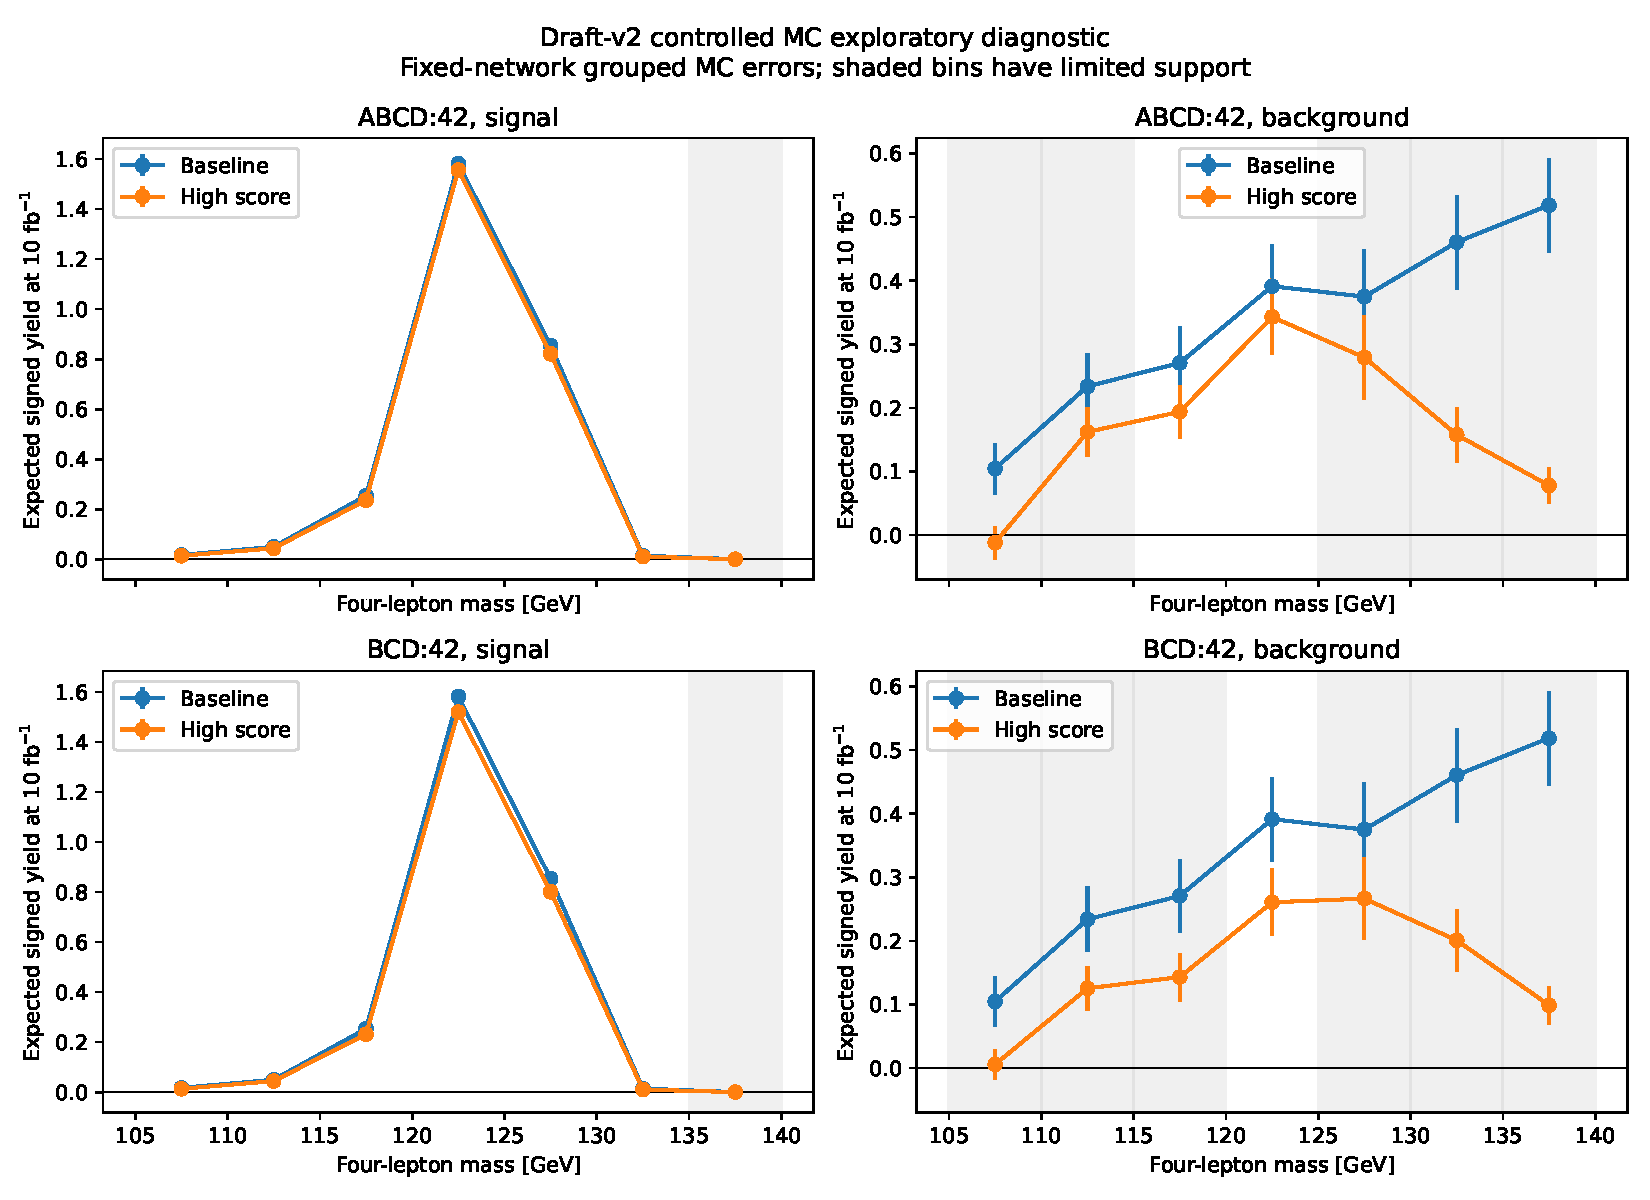
\includegraphics[width=.92\linewidth]{figures/draft001/mass-yields.pdf}
\caption{draft001 最终评估的带符号质量谱。上排为 ABCD，下排为 BCD，均使用种子 42。
蓝色圆点为基线，橙色菱形为高分事件；左列为信号，右列为背景。每点代表一个 5 GeV 箱，
连线仅作视觉引导，不代表连续质量模型。纵轴为 $10\,\mathrm{fb}^{-1}$ 下的预期产额，信号与背景刻度不同。
误差棒采用按事件组计算的 MC 方差。阴影按下述标准标记统计支持不足的区域；负产额保留。}
\label{fig:yields}
\end{figure}



\textbf{信号位置。} 模拟信号集中在 125 GeV 附近，两条筛选后曲线基本保留该区域。
网络不改变单个事件的质量；分布变化来自对基线事件的子集选择。粗分箱不能证明峰位移动、
探测器分辨率改善或希格斯物理宽度变化。

\textbf{背景分布。} 背景覆盖整个质量窗口，筛选前已不均匀。不同质量区域的压低程度不同，
高质量尾部尤其明显。因此，信号在视觉上更突出需要从两方面解释：背景减少了多少，以及剩余背景如何分布。
下一节分别归一化的谱形用于回答第二个问题。
\FloatBarrier
\clearpage
\subsection{归一化谱形：去除总量变化后的比较}
图~\ref{fig:shapes} 将每个过程、每种选择分别除以其自身带符号总产额，从比较中去除总体产额变化。
表~\ref{tab:fractions} 使用固定质量区域量化主要可见变化。

\begin{figure}[H]
\centering
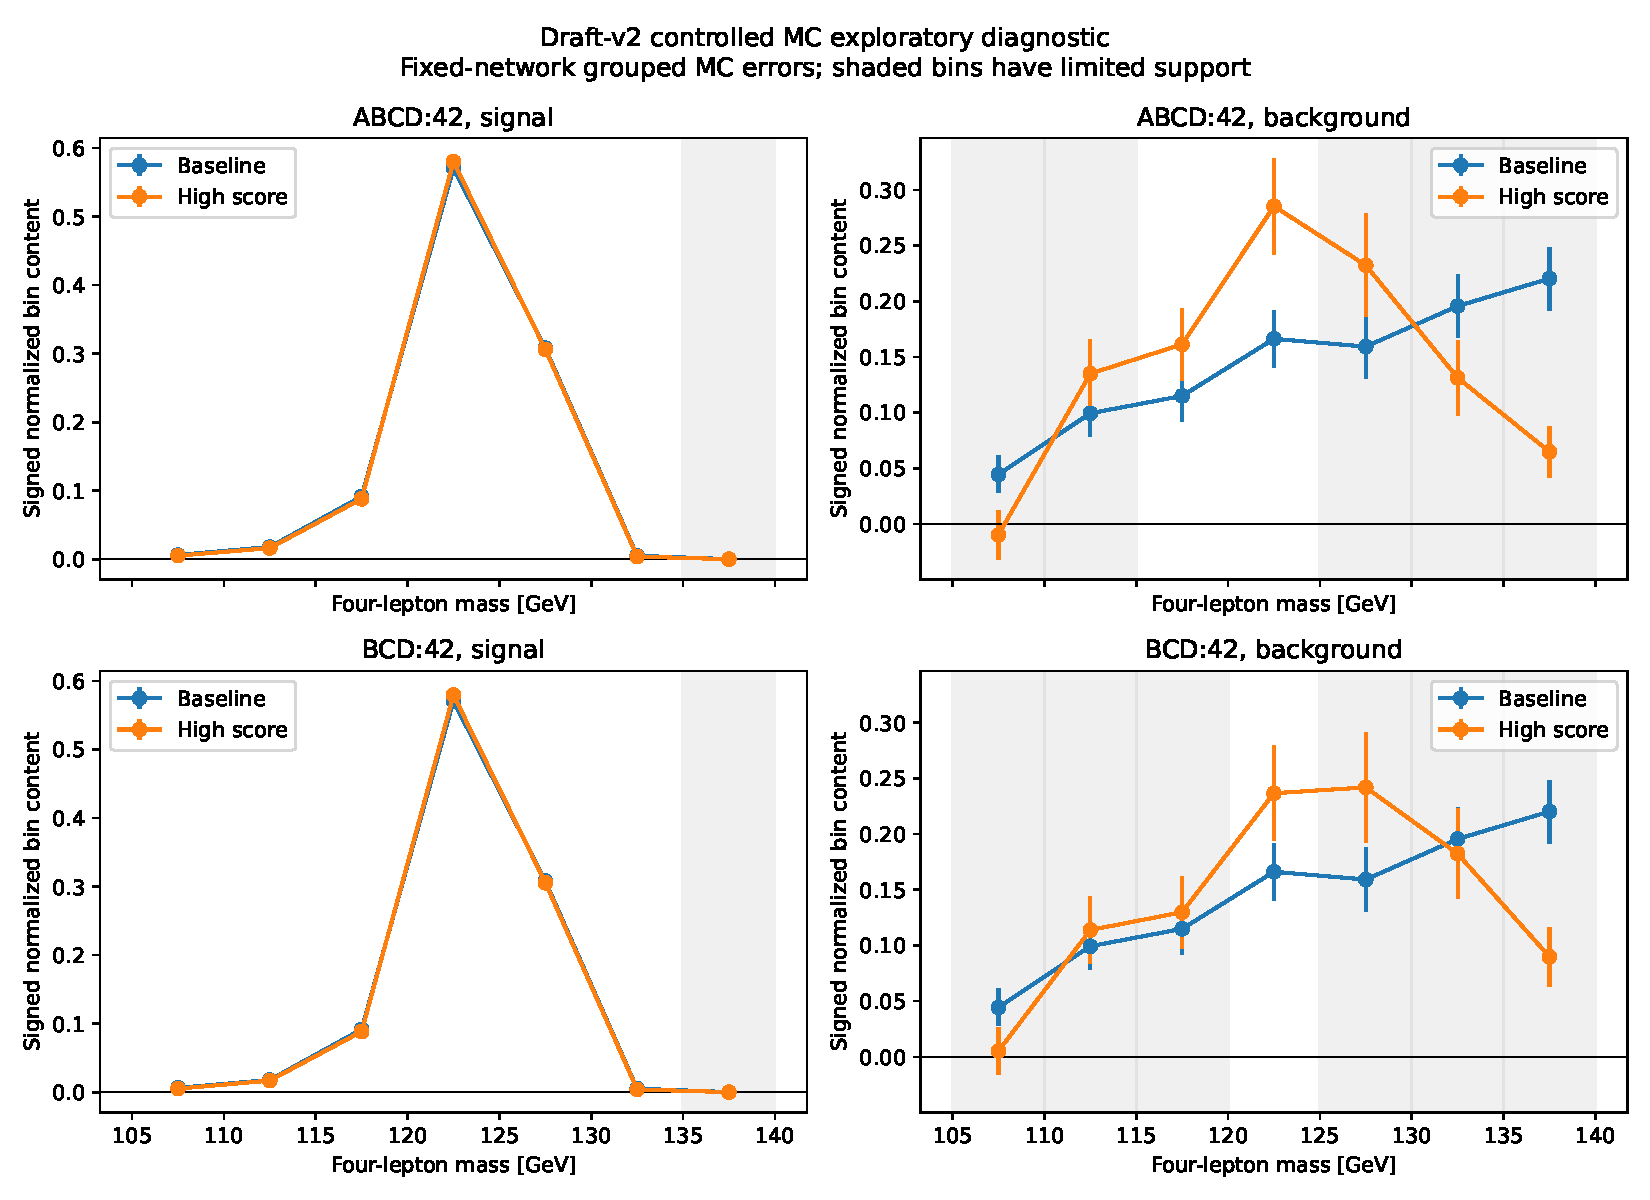
\includegraphics[width=.82\linewidth]{figures/draft001/mass-shapes.pdf}
\caption{与图~\ref{fig:yields} 使用相同事件和阈值、分别归一化后的筛选前后质量谱形。
每个箱除以其曲线自身为正的带符号总产额。误差传播包括共享归一化；筛选前后也共享事件。
带符号归一化谱形不一定是概率密度。保留阴影箱和负值箱，不作平滑、裁剪或重新分箱。}
\label{fig:shapes}
\end{figure}

\begin{table}[H]
\caption{固定质量区域内的带符号产额占各自曲线总产额的比例（\%）。
数值为描述性点估计，未展示不确定度，不能据此判定筛选前后差异的统计显著性。}
\label{tab:fractions}
\centering
\small
\begin{tabular}{llrrr}
\toprule
过程 & 区域（GeV） & 筛选前 & ABCD 高分 & BCD 高分 \\
\midrule
信号 & $[120,130)$ & 87.9 & 88.6 & 88.5 \\
背景 & $[120,130)$ & 32.5 & 51.8 & 47.9 \\
背景 & $[135,140)$ & 22.0 & 6.5 & 9.0 \\
\bottomrule
\end{tabular}
\end{table}

\textbf{解释。} 信号仍集中于其主要质量区域；背景在该区域的相对占比上升，而高质量尾部占比下降。
这描述性地表明，即使不显式输入 $m_{4\ell}$，已冻结的选择仍与质量有关。
它不能确定唯一负责的输入特征，也不能证明背景存在物理共振。
\FloatBarrier
\textbf{统计支持标记。} 若某质量箱的基线或高分样本满足任一条件，则标为阴影：无事件组；
带符号产额 $Y$ 或分组方差 $V$ 非正；带符号有效计数 $N_{\rm eff}=Y^2/V<20$；
或抵消比 $\rho=|Y|/\sum_i|w_i|<0.2$。其中 $w_i$ 为事件的评估产额权重，
$V$ 为各物理事件组产额贡献的平方和。阴影属于统计支持诊断，并非置信带。
图~\ref{fig:shapes} 的归一化谱形采用相同标准。

\textbf{限制。} ABCD 筛选后的背景在 $[105,110)$ GeV 箱中为负；若干背景箱和信号高质量尾部的统计支持不足。
共享事件与归一化产生的相关性，使图中误差不能视为独立测量。误差以固定网络和阈值为条件，
不包含阈值估计、独立重训练及覆盖率不确定度。
\FloatBarrier

\section{输入组删减对标称区间的影响}

\subsection{区间构造与比较规则}

完整比较对 ABCD、BCD、ACD、ABD、ABC 五种表示分别使用种子 42、43、44 训练，
得到 15 个标称区间；另有一个共享包容计数参考，不使用训练分类器，也没有训练种子变化。
这些结果均沿用既有报告中的有效数值状态。

信号强度 $\mu$ 表示预期信号产额的缩放倍数。比较指标
$W_{68}=\mu_{\rm upper}-\mu_{\rm lower}$ 是指定模型下标称 68\% 信号强度区间的宽度。
这里关注的是相同分析约定下的区间宽度，不能将较小的数值直接解释为已验证的测量精度提升。

每个区间采用其自身模型在注入 $\mu=1$ 时生成的 Asimov 期望观测，即以模型期望值代替一次随机观测。
T1 似然对有限模板统计的干扰参数作剖面化；在 $0\leq\mu\leq20$ 内，
区间端点由剖面似然比统计量达到一个自由度 $\chi^2$ 分布的渐近 68\% 分位数确定。
高分和低分两个类别均进入似然，各自在单一质量区间 $[105,140)$ GeV 上积分；
这不是对图中七个质量箱进行质量峰拟合。标称 68\% 不代表重复抽样覆盖率已经校准。

\subsection{五种表示与种子内配对比较}
\begin{table}[H]
\caption{五种表示与共享包容计数参考的标称区间宽度。五种训练表示以三个固定种子的中位数汇总；包容计数参考只有一个共享结果，不取种子中位数。种子不是重复的独立 MC 样本。}
\label{tab:widths}
\centering
\begin{tabular}{llr}
\toprule
输入表示 & 去掉的输入组 & $W_{68}$（模型取中位数） \\
\midrule
ABCD & 无 & 1.464392 \\
BCD & A & 1.474847 \\
ACD & B & 1.467509 \\
ABD & C & 1.505681 \\
ABC & D & 1.452977 \\
包容计数参考 & 不使用训练分类器 & 1.638845 \\
\bottomrule
\end{tabular}
\end{table}四项比较先在每个种子内计算
$\Delta W_G=W_{68}(\mathrm{ABCD}\setminus G)-W_{68}(\mathrm{ABCD})$，再汇总。
去掉 C 使三个种子的区间均变宽，中位数为 $\Delta W_C=0.046283$。
A、B、D 的差值在不同种子间改变符号。ABC 在五种表示中的中位宽度最小，
但这不足以确立普遍最优的输入组合或已证实的精度提升。
这里的删组差值在同一个种子内先作相减，再对三个差值取中位数。
它一般不等于分别取两组宽度中位数后再相减；按种子配对才能保持原比较规则。
C 组包含 $p_{T,4\ell}$ 和两个轻子对之间的方位角差；当前结果描述这一整组的删减效果，
不单独识别某个变量的因果贡献。

\FloatBarrier

\section{差异的稳定性与统计可靠性}

\subsection{有限 MC 与阈值重估}
\textbf{补充统计评估。} 已完成 200 次配对事件组重抽样（bootstrap，含阈值重估诊断）及
24,000 次模型自生成伪实验（model-self Toys），均具有有效数值状态。
固定网络并重估阈值时，$\Delta W_C$ 和 $\Delta W_D$ 的 95\% 重抽样百分位范围分别为
$[0.0101,0.0711]$ 和 $[-0.0384,0.0055]$，A、B 的范围均跨零。
删去 C 的变宽现象较稳健；删去 D 的改善尚不稳健。
配对事件组重抽样让各模型在相同的评估重抽样上比较；阈值重估诊断则在固定网络下，
按原规则从重抽样验证背景重新计算阈值。重估阈值只属于诊断副本，不替换原来冻结的阈值。
因此，它考察有限 MC 和阈值估计带来的变化，但不包含重新训练网络的全部不确定性。

\subsection{模型自生成覆盖率与欠覆盖}
\textbf{解释状态。} 这些结果属于探索性、非独立 MC 结果。重新划分后，研究仍使用先前已使用过的源事件。
区间以自身模板作为期望观测；在 $\mu=1$ 的 model-self 检验中，16 个候选的标称 68\% 区间覆盖率为
60.4\%--67.2\%，存在欠覆盖，尚未独立校准。重抽样范围条件于既有检查点，
不包含独立重训练及完整模型选择的不确定性，不是已校准的置信区间。种子变化范围也不是置信区间。
项目属于教育与技术研究，不是 ATLAS/CMS 官方结果、希格斯发现或物理测量。
\subsection{当前诊断的解释边界}

模型自生成伪实验以各自模板作为生成模型，检查该模型内部的区间行为；它不是独立物理参考。
同一源事件重新划分后也不会变成新的独立总体。
所以，已有数值完成状态和重抽样方向稳定性不能替代独立覆盖率校准、物理适用性验证或完整模型选择不确定性研究。

\section{当前结论与下一步优先级}

现有证据支持三点有限判断。第一，两个示例选择都能在保留大部分信号产额的同时减少背景，
但需要同时报告背景的质量谱形变化。第二，删去 C 组的标称区间变宽方向在当前三个种子及固定网络重抽样中较稳健，
其余组不能据当前排序确定普遍优劣。第三，model-self 诊断显示欠覆盖，标称区间缩窄不等于已确认的精度提升。

下一步应先明确哪些结论受物理样本和选择适用性限制，哪些受统计校准限制，再决定是否增加研究。

优先核实样本生产配置、发布前筛选、项目选择条件的外部依据以及物理权重的适用性。
统计方面应继续研究低计数区间构造与覆盖率校准；独立 assessment 和完整 T2 仍属于按需后续研究，
不能将现有 model-self 诊断视为它们已完成。

\clearpage
\appendix

\section{字段、重建与输入约定}\label{app:fields}

\subsection{模拟与发布范围}
\textbf{模拟与发布。} 一般模拟链为：设定物理过程并生成硬散射，模拟粒子簇射与强子化，
模拟探测器响应，再重建电子、缪子等对象，最后预筛选并发布 ROOT 文件。
这里使用公开的轻子对象字段构造候选，不使用生成器真值四动量；后文“重建”指本项目的四动量组合。
两份样本的生成器版本、簇射和探测器模拟配置仍待生产记录核实，不能沿用参考论文的配置。
CERN 记录只确认发布前施加宽松对象和事件选择、保留至少四个电子或缪子；其具体动量、接受度及品质阈值尚未确认。
故本项目研究的是已预筛选的总体，再施加本项目的共同筛选，不能由表~\ref{tab:population} 推算相对全部生成事件的接受效率。
\subsection{读取字段}
\textbf{事件结构。} \texttt{mini} 树的一个 entry 是一条事件记录，branch 是其中一个字段。
下表列出本项目读取的全部 19 个分支，\emph{不是原始文件的完整分支清单，也不是 19 维网络输入}。
前七个字段为标量，其余为向量；例如 \texttt{lep\_n=4} 时，各轻子向量均含四个元素，相同下标对应同一轻子。

\begingroup
\small
\renewcommand{\arraystretch}{1.13}
\begin{tabularx}{\linewidth}{@{}p{.62\linewidth}Y@{}}
\toprule
读取的分支 & 含义与存储单位 \\
\midrule
\texttt{runNumber, eventNumber, channelNumber} & 事件／样本标识（整数） \\
\texttt{mcWeight; trigE, trigM; lep\_n} & 生成器权重；触发布尔值；轻子数 \\
\texttt{lep\_pt, lep\_eta, lep\_phi, lep\_E} & $p_T$、$\eta$、$\phi$、能量；动量和能量为 MeV，角度为弧度 \\
\texttt{lep\_charge, lep\_type} & 电荷和粒子类型（整数向量） \\
\texttt{lep\_isTightID, lep\_trigMatched} & 鉴别和触发匹配标志（布尔向量） \\
\texttt{lep\_ptcone30, lep\_etcone20} & 径迹／量能器隔离量（MeV） \\
\texttt{lep\_z0; lep\_tracksigd0pvunbiased} & $z_0$（mm）；$d_0/\sigma(d_0)$（无量纲） \\
\bottomrule
\end{tabularx}
\endgroup

运动学、隔离及碰撞参数字段为浮点向量。使用时将 MeV 换算为 GeV；带符号权重转换为预期产额的方法见第~\ref{sec:weights} 节。
上述字段映射来自项目输入配置及此前 ROOT 元数据核对；这不补足尚缺的生产链证据。
\subsection{四动量重建与输入分组}
\textbf{从轻子字段到候选。} 对通过品质筛选的轻子，先将动量和能量换算为 GeV，并按 $p_T$ 降序编号。
以 $c=1$，由公开的 $(p_T,\eta,\phi,E)$ 构造四动量：
\[
 p^\mu=(E,p_x,p_y,p_z),\qquad
 p_x=p_T\cos\phi,\quad p_y=p_T\sin\phi,\quad p_z=p_T\sinh\eta.
\]
电荷和味道确定 SFOS 配对。在本项目 $2e2\mu$ 道中，电子对和缪子对给出唯一的两对；
质量更接近 $91.1876\gev$ 的一对记为 $Z_1$，另一对记为 $Z_2$。
文献的 $m_{12},m_{34}$ 即代码中的 \texttt{mZ1,mZ2}；$Z_1$ 不固定指电子对，也不按 $p_T$ 编号。
相加得到 $P_j=p_{j^-}+p_{j^+}$、$Q=P_1+P_2$，再计算
\[
 m_{Zj}=\sqrt{P_j^2},\qquad m_{4\ell}=\sqrt{Q^2},\qquad
 p_{T,4\ell}=\sqrt{Q_x^2+Q_y^2}.
\]
这一步组合已有轻子对象，不重新模拟探测器。重建质量谱可能受到辐射、探测器响应及选择影响，
其宽度不能直接解释为希格斯本征宽度。\textbf{输入来源。} A 组直接取排序后的 $p_T,\eta$；B、C 组由上述四动量计算。
$\Delta R$ 使用同一对内两轻子的 $\eta,\phi$，方位角差先折回 $[-\pi,\pi)$；
\texttt{deltaPhi\_ZZ} 则是两个轻子对方位角差的绝对值。以下 19 维输入不是 ROOT 中另外 19 个现成字段。\begin{table}[H]
\caption{输入变量分组及其物理含义。动量和质量使用 GeV，方位角使用弧度。}
\label{tab:features}
\small
\renewcommand{\arraystretch}{1.12}
\begin{tabularx}{\linewidth}{@{}p{.05\linewidth}p{.43\linewidth}cY@{}}
\toprule
组 & 代码变量 & 维数 & 物理含义 \\
\midrule
A & \texttt{lep1\_pt}--\texttt{lep4\_pt}；\texttt{lep1\_eta}--\texttt{lep4\_eta} & 8 &
单轻子的横动量和赝快度，描述动量尺度及相对束流的方向。 \\
B & \texttt{mZ1}, \texttt{mZ2}；\texttt{deltaR\_Z1}, \texttt{deltaR\_Z2} & 4 &
两个轻子对的质量，以及各对内部的角分离 $\Delta R=\sqrt{(\Delta\eta)^2+(\Delta\phi)^2}$。 \\
C & \texttt{pt4l}, \texttt{deltaPhi\_ZZ} & 2 &
四轻子系统的横动量，以及两个轻子对之间的方位角差绝对值。 \\
D & \texttt{cos\_theta\_star}, \texttt{cos\_theta\_1}, \texttt{cos\_theta\_2}；
\texttt{phi\_decay\_planes}, \texttt{phi\_production\_plane} & 5 &
一个产生角余弦、两个衰变极角余弦，以及描述衰变平面与产生平面相对取向的两个角。 \\
\bottomrule
\end{tabularx}
\end{table}
\subsection{五个角度的约定}
\textbf{五个角度的计算方法。} D 组先作洛伦兹变换。在四轻子静止系中，
$\cos\theta^*$ 是 $Z_1$ 与变换后的实验室正束流方向的夹角余弦；
$\cos\theta_1,\cos\theta_2$ 分别在各自轻子对静止系中，取负轻子方向与另一轻子对反方向的夹角余弦。
两个平面角在四轻子静止系计算：用负、正轻子动量的叉积定义各衰变平面法向量，
用正束流方向与 $Z_1$ 方向定义产生平面法向量；绕 $Z_1$ 轴用有向角分别比较两个衰变平面、产生平面与第一衰变平面。
角度范围为 $[-\pi,\pi)$，余弦范围为 $[-1,1]$，各模型沿用同一约定。
\FloatBarrier

\section{完整选择条件与物理归一化}\label{app:cuts}

\subsection{共同选择的执行顺序}
\begin{table}[H]
\caption{共同筛选的执行顺序。动量与质量单位为 GeV，分支含义见附录~\ref{app:fields}。}
\label{tab:cuts}
\small
\renewcommand{\arraystretch}{1.1}
\begin{tabularx}{\linewidth}{@{}p{.23\linewidth}Y@{}}
\toprule
步骤 & 实际条件及目的 \\
\midrule
\textbf{事件触发} & \texttt{trigE} 或 \texttt{trigM} 为真，要求事件通过电子或缪子触发。 \\
\midrule
\textbf{轻子品质} & 依次执行以下条件，每步至少保留四个轻子，以筛出符合要求的提示轻子候选： \\
味道、鉴别 & $|\texttt{lep\_type}|\in\{11,13\}$；\texttt{lep\_isTightID=true}。 \\
径迹、量能器隔离 & $p_T>0$；依次要求 \texttt{lep\_ptcone30}/\texttt{lep\_pt}$<0.3$、
\texttt{lep\_etcone20}/\texttt{lep\_pt}$<0.3$，抑制周围活动较多的对象。 \\
横向、纵向碰撞参数 & $|d_0/\sigma(d_0)|<$ 5（电子）或 3（缪子）；
$|z_0/\cosh\eta|<0.5$ mm，限制相对主顶点的位移。 \\
\midrule
\textbf{四轻子候选} & 以下条件依次定义共同分析总体： \\
多重数、触发匹配 & 品质筛选后恰好四个轻子；至少一个 \texttt{lep\_trigMatched=true}。
原始 \texttt{lep\_n} 可以大于四。 \\
排序动量、接受度 & 按 $p_T$ 降序，依次 $\geq20,15,10,7$；
电子 $|\eta|<2.47$、缪子 $|\eta|<2.7$，限定运动学及探测器接受范围。 \\
电荷、配对 & 总电荷为零；存在两个互不重叠的同味异号（SFOS）对，构造 $ZZ^*$ 候选。 \\
轻子对质量 & 所有 SFOS 质量 $>5$；$50<m_{Z1}<106$、$12<m_{Z2}<115$，排除低质量对并限定候选。 \\
四轻子质量、末态 & $105\leq m_{4\ell}<140$；随后要求两个电子和两个缪子，限定本项目研究范围。 \\
\bottomrule
\end{tabularx}
\end{table}
\Needspace{12\baselineskip}
\subsection{文献依据与项目差异}
\textbf{物理来源及项目改动。} ATLAS 13 TeV 分析\cite{ATLAS13} 第 5.1--5.2 节支持接受度、
前三个动量尺度、SFOS 配对、$Z$ 质量窗口及横向碰撞参数条件的物理动机；
$12\gev$ 的次主导质量下限适用于这里的 $m_{4\ell}<140\gev$。以下差异须保留：
\begin{itemize}[itemsep=1pt,topsep=2pt]
\item 文献使用宽松电子鉴别及详细缪子要求；本项目统一使用 tight-ID，工作点等价性未确认。
\item 本项目动量阈值允许取等号，第四轻子统一 $p_T\geq7$；文献分别要求电子 $E_T>7$、缪子 $p_T>5$，部分缪子另有要求。
\item 本项目两种隔离均 $<30\%$；文献径迹隔离 $<15\%$，量能器隔离电子 $<20\%$、缪子 $<30\%$，且有额外锥及修正规定。
\item 本项目仅取恰好四个合格轻子的 $2e2\mu$ 道；未复现文献的多候选、角分离等完整程序。该道的 $Z$ 窗口已比 $5\gev$ 条件更严格。
\end{itemize}
官方教育示例\cite{HZZCuts,HZZAnalysis}支持部分多重数、电荷、味道和动量规则，但其隔离函数调用已注释掉。
Run-1 文献\cite{ATLASRun1}支持触发匹配原则。tight-ID 工作点与 $|z_0\sin\theta|<0.5$ mm 的确切外部依据仍待核实，
本报告将其列为项目固定选择，不声称复现已发表测量。
\subsection{物理权重的归一化}
\label{app:weights}
\textbf{从模拟事件数到预期产额。} 每个事件的物理权重为
\[
 w_i^{\rm phys}=\frac{\mathcal L\,\sigma_{\rm eff}}{S_{\rm gen}}\,w_i^{\rm gen},
 \qquad \mathcal L=10^4\,\mathrm{pb}^{-1},\quad w_i^{\rm gen}=\texttt{mcWeight}.
\]
这里 $\sigma_{\rm eff}$ 为配置中的有效截面，$S_{\rm gen}$ 为样本归一化用的生成器权重和，
不是公开条目数或筛选后事件数。官方固定版本参数表\cite{SampleInfo}给出：
信号 $(\sigma_{\rm eff},S_{\rm gen})=(0.0060239\,\mathrm{pb},27881776.6536)$，
背景为 $(1.2578\,\mathrm{pb},7538705.8077)$，与项目配置一致。
项目不再另乘 $k$ 因子或过滤效率（配置均为 1）；有效截面中分支比与过滤效率的具体分解仍待生产说明核实，不能重复乘入。
当前也未乘堆积、轻子和触发尺度因子，与官方示例\cite{HZZAnalysis}有别，不能据此复现其产额。
\FloatBarrier

\section{样本计数与训练细节}

\subsection{公开输入及三个子集的计数}
\begin{table}[H]
\caption{公开输入与本项目共同筛选后的数量。首行为 ROOT 条目数；其后为 draft001 的物理事件组数，
已核对所选条目与事件组一一对应。后三行是共同筛选总体的互斥划分。}
\label{tab:population}
\centering
\small
\begin{tabular}{lrrr}
\toprule
阶段 & 信号 & 背景 & 合计 \\
\midrule
公开 ROOT 输入（项目筛选前） & 164,716 & 554,279 & 718,995 \\
共同筛选后（全部子集） & 45,083 & 3,593 & 48,676 \\
\quad 训练子集 & 27,026 & 2,175 & 29,201 \\
\quad 验证子集 & 9,008 & 720 & 9,728 \\
\quad 最终评估子集 & 9,049 & 698 & 9,747 \\
\bottomrule
\end{tabular}
\end{table}
这些计数沿用既有 prepare 身份核对，不是逐条筛选计数，也不包含发布前被滤掉的事件。

\subsection{网络结构与训练配置}
\label{app:network}
\textbf{固定结构与参数。} 全连接网络为
$d_{\rm in}\to64\to64\to32\to1$，三个隐藏层均有 LayerNorm 和 SiLU，前两个隐藏层后有 0.1 Dropout，
输出经 sigmoid 转为分数。ABCD/BCD 输入维数为 19/11；学习率 $10^{-3}$，权重衰减 $10^{-4}$，
批量 1024，使用 CPU float32。
\subsection{阈值公式与教学示例}
\label{app:threshold}
令 $a_i=|w_i|$ 为其绝对物理权重，依次累计 $a_i$；第一次达到总绝对权重一半的分数就是阈值：
\[
 k=\min\left\{j:\sum_{i=1}^{j}a_{(i)}\geq\frac12\sum_i a_i\right\},
 \qquad t=s_{(k)}.
\]
下标 $(i)$ 表示按分数排序。此处不作分数插值；评估时 $s\geq t$ 为高分类别，$s<t$ 为低分类别，
同分事件整体进入同一类别。\textbf{教学示例（非实际运行数据）。} 假设五个验证背景事件的有序分数为
$0.10,0.30,0.60,0.80,0.90$，对应绝对权重为 $1,2,1,4,2$。
总权重为 10，一半为 5；累计权重依次为 $1,3,4,8,10$，首次达到 5 的位置对应 $t=0.80$。
因此分数 0.80 和 0.90 进入高分类别，其绝对权重占比为 $6/10=60\%$。
离散权重和同分事件使该比例不必恰好为 50\%，更不要求评估集的\emph{带符号}背景保留率为 50\%。
\FloatBarrier

\section{结果来源与修订范围}\label{app:provenance}
\textbf{本地结果来源。} 标称区间、产额与质量谱结果及两幅图仍来自
\nolinkurl{runs/h4l-draft-v2-draft001/report/}，并关联已完成的准备、冻结和评估产物。
英文报告记录：报告文件大小与 SHA-256 已对照清单核对，两份图的副本与报告原图逐字节一致。
补充统计结果来自 \nolinkurl{runs/h4l-draft-v2-validation001/report/}。
详细身份记录见 \nolinkurl{paper/draft-v2/DRAFT001-EVIDENCE.md}；
冻结协议为 \nolinkurl{config/protocols/h4l_draft_v2.json}。
本次只重组已有中文报告并改写说明，未新增科学结果。标称数值与两幅质量谱图沿用 draft001，
统计诊断沿用 validation001；原有结果身份、协议与资格保持不变。
此前记录的哈希核验属于历史溯源，本次仅检查文稿数值保留、引用及编译排版，未重新审计运行产物。
未读取事件载荷、重新训练、评分、拟合或生成伪实验。

文献与样本参数依据沿用原报告的 2026 年 10 月 30 日及 11 月 1 日核对记录，本次未新增外部文献核查。
CERN 发布记录说明该数据集用于教育，不适用于科学出版；本报告保持教育与技术研究范围。
DSID 生产配置、发布前精确筛选及完整官方分支说明仍待对应版本来源核实。

\begingroup
\small
\renewcommand{\refname}{本报告参考文献}
\begin{thebibliography}{9}
\bibitem{OpenData}
ATLAS Collaboration, \emph{ATLAS 13 TeV samples collection at least four leptons
(electron or muon), for 2020 Open Data release} (2020).
\href{https://opendata.cern.ch/record/15005}{CERN Open Data record 15005},
\href{https://doi.org/10.7483/OPENDATA.ATLAS.2Y1T.TLGL}{doi:10.7483/OPENDATA.ATLAS.2Y1T.TLGL}.
两份模拟数据及发布前宽松预筛选说明的来源；使用限制见记录声明。

\bibitem{ATLAS13}
ATLAS Collaboration, \emph{Measurement of the Higgs boson coupling properties in
the $H\to ZZ^*\to4\ell$ decay channel at $\sqrt{s}=13$ TeV with the ATLAS detector},
JHEP \textbf{03} (2018) 095.
\href{https://doi.org/10.1007/JHEP03(2018)095}{doi:10.1007/JHEP03(2018)095};
\href{https://arxiv.org/pdf/1712.02304v2#page=8}{arXiv:1712.02304v2，第 5.1--5.2 节，第 8--9 页}。
附录~\ref{app:cuts} 中筛选与工作点比较的来源。

\bibitem{HZZCuts}
ATLAS Open Data outreach tools, \emph{HZZCuts.py}，版本
\nolinkurl{8ad2015be6d350060c3a183aff5802570bc9ada4}。
\href{https://github.com/atlas-outreach-data-tools/atlas-outreach-Python-uproot-framework-13tev/blob/8ad2015be6d350060c3a183aff5802570bc9ada4/HZZCuts.py#L2-L33}{固定版本源码，第 2--33 行}。
多重数、电荷、部分动量条件、味道及可选隔离定义。

\bibitem{HZZAnalysis}
ATLAS Open Data outreach tools, \emph{HZZAnalysis.py}，版本同文献~\cite{HZZCuts}。
\href{https://github.com/atlas-outreach-data-tools/atlas-outreach-Python-uproot-framework-13tev/blob/8ad2015be6d350060c3a183aff5802570bc9ada4/HZZAnalysis.py#L140-L168}{固定版本源码，第 140--168 行}。
事件权重因子、实际施加的筛选及已注释的隔离调用。

\bibitem{ATLASRun1}
ATLAS Collaboration, \emph{Measurements of Higgs boson production and couplings
in the four-lepton channel in $pp$ collisions at center-of-mass energies of
7 and 8 TeV with the ATLAS detector}, Phys.~Rev.~D \textbf{91}, 012006 (2015).
\href{https://doi.org/10.1103/PhysRevD.91.012006}{doi:10.1103/PhysRevD.91.012006};
\href{https://arxiv.org/pdf/1408.5191v3#page=7}{arXiv:1408.5191v3，第 5.1 节，印刷页码第 6--7 页}。
触发匹配原则的参考；不声称其详细阈值和工作点与本项目相同。
\bibitem{SampleInfo}
ATLAS Open Data outreach tools, \emph{infofile.py}，版本同文献~\cite{HZZCuts}。
\href{https://github.com/atlas-outreach-data-tools/atlas-outreach-Python-uproot-framework-13tev/blob/8ad2015be6d350060c3a183aff5802570bc9ada4/infofile.py}{固定版本样本参数表}。
\texttt{ggH125\_ZZ4lep} 与 \texttt{llll} 条目的 DSID、\texttt{xsec} 和 \texttt{sumw}；
不提供完整生成器或探测器模拟配置。
\end{thebibliography}
\endgroup
\end{document}
